% !TeX TS-program = txs:///duck
\documentclass{standalone}
\usepackage{tikzducks}

\definecolor{pskin}{RGB}{255,200,184}
\definecolor{phair}{RGB}{249,249,139}

\begin{document}
	
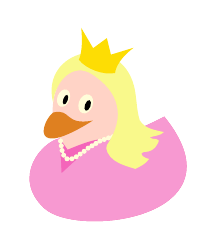
\begin{tikzpicture}
	\duck[
		body=pskin!80!white,
		longhair=phair,
		tshirt=magenta!60!white,
		jacket=magenta!40!white,
		necklace=white!85!yellow
	]
	\path (0.7,2) rectangle (1.4,2.55);
	\fill[yellow!80!orange,rotate=-10,xshift=-11,yshift=5] \duckpathcrown;
\end{tikzpicture}

\end{document}